\begin{fact} \label{tri-one-side-fixed}
	Considérons tous les triangles de périmètre fixé $p$, et ayant tous un côté en commun.
	Parmi tous ces triangles, un seul est d'aire maximale, c'est le triangle isocèle ayant pour base le côté commun.
\end{fact}


\begin{proof}
	Soit $ABC$ un triangle de périmètre $p$, et fixons le côté $[AB]$. 
	Pour tout point $M$ sur la parallèle à $(AB)$ passant par $C$, nous savons que $\area{ABM} = \area{ABC}$. Notons alors $O$ le point sur cette parallèle tel que $ABO$ soit isocèle en $O$.

	\begin{center}
		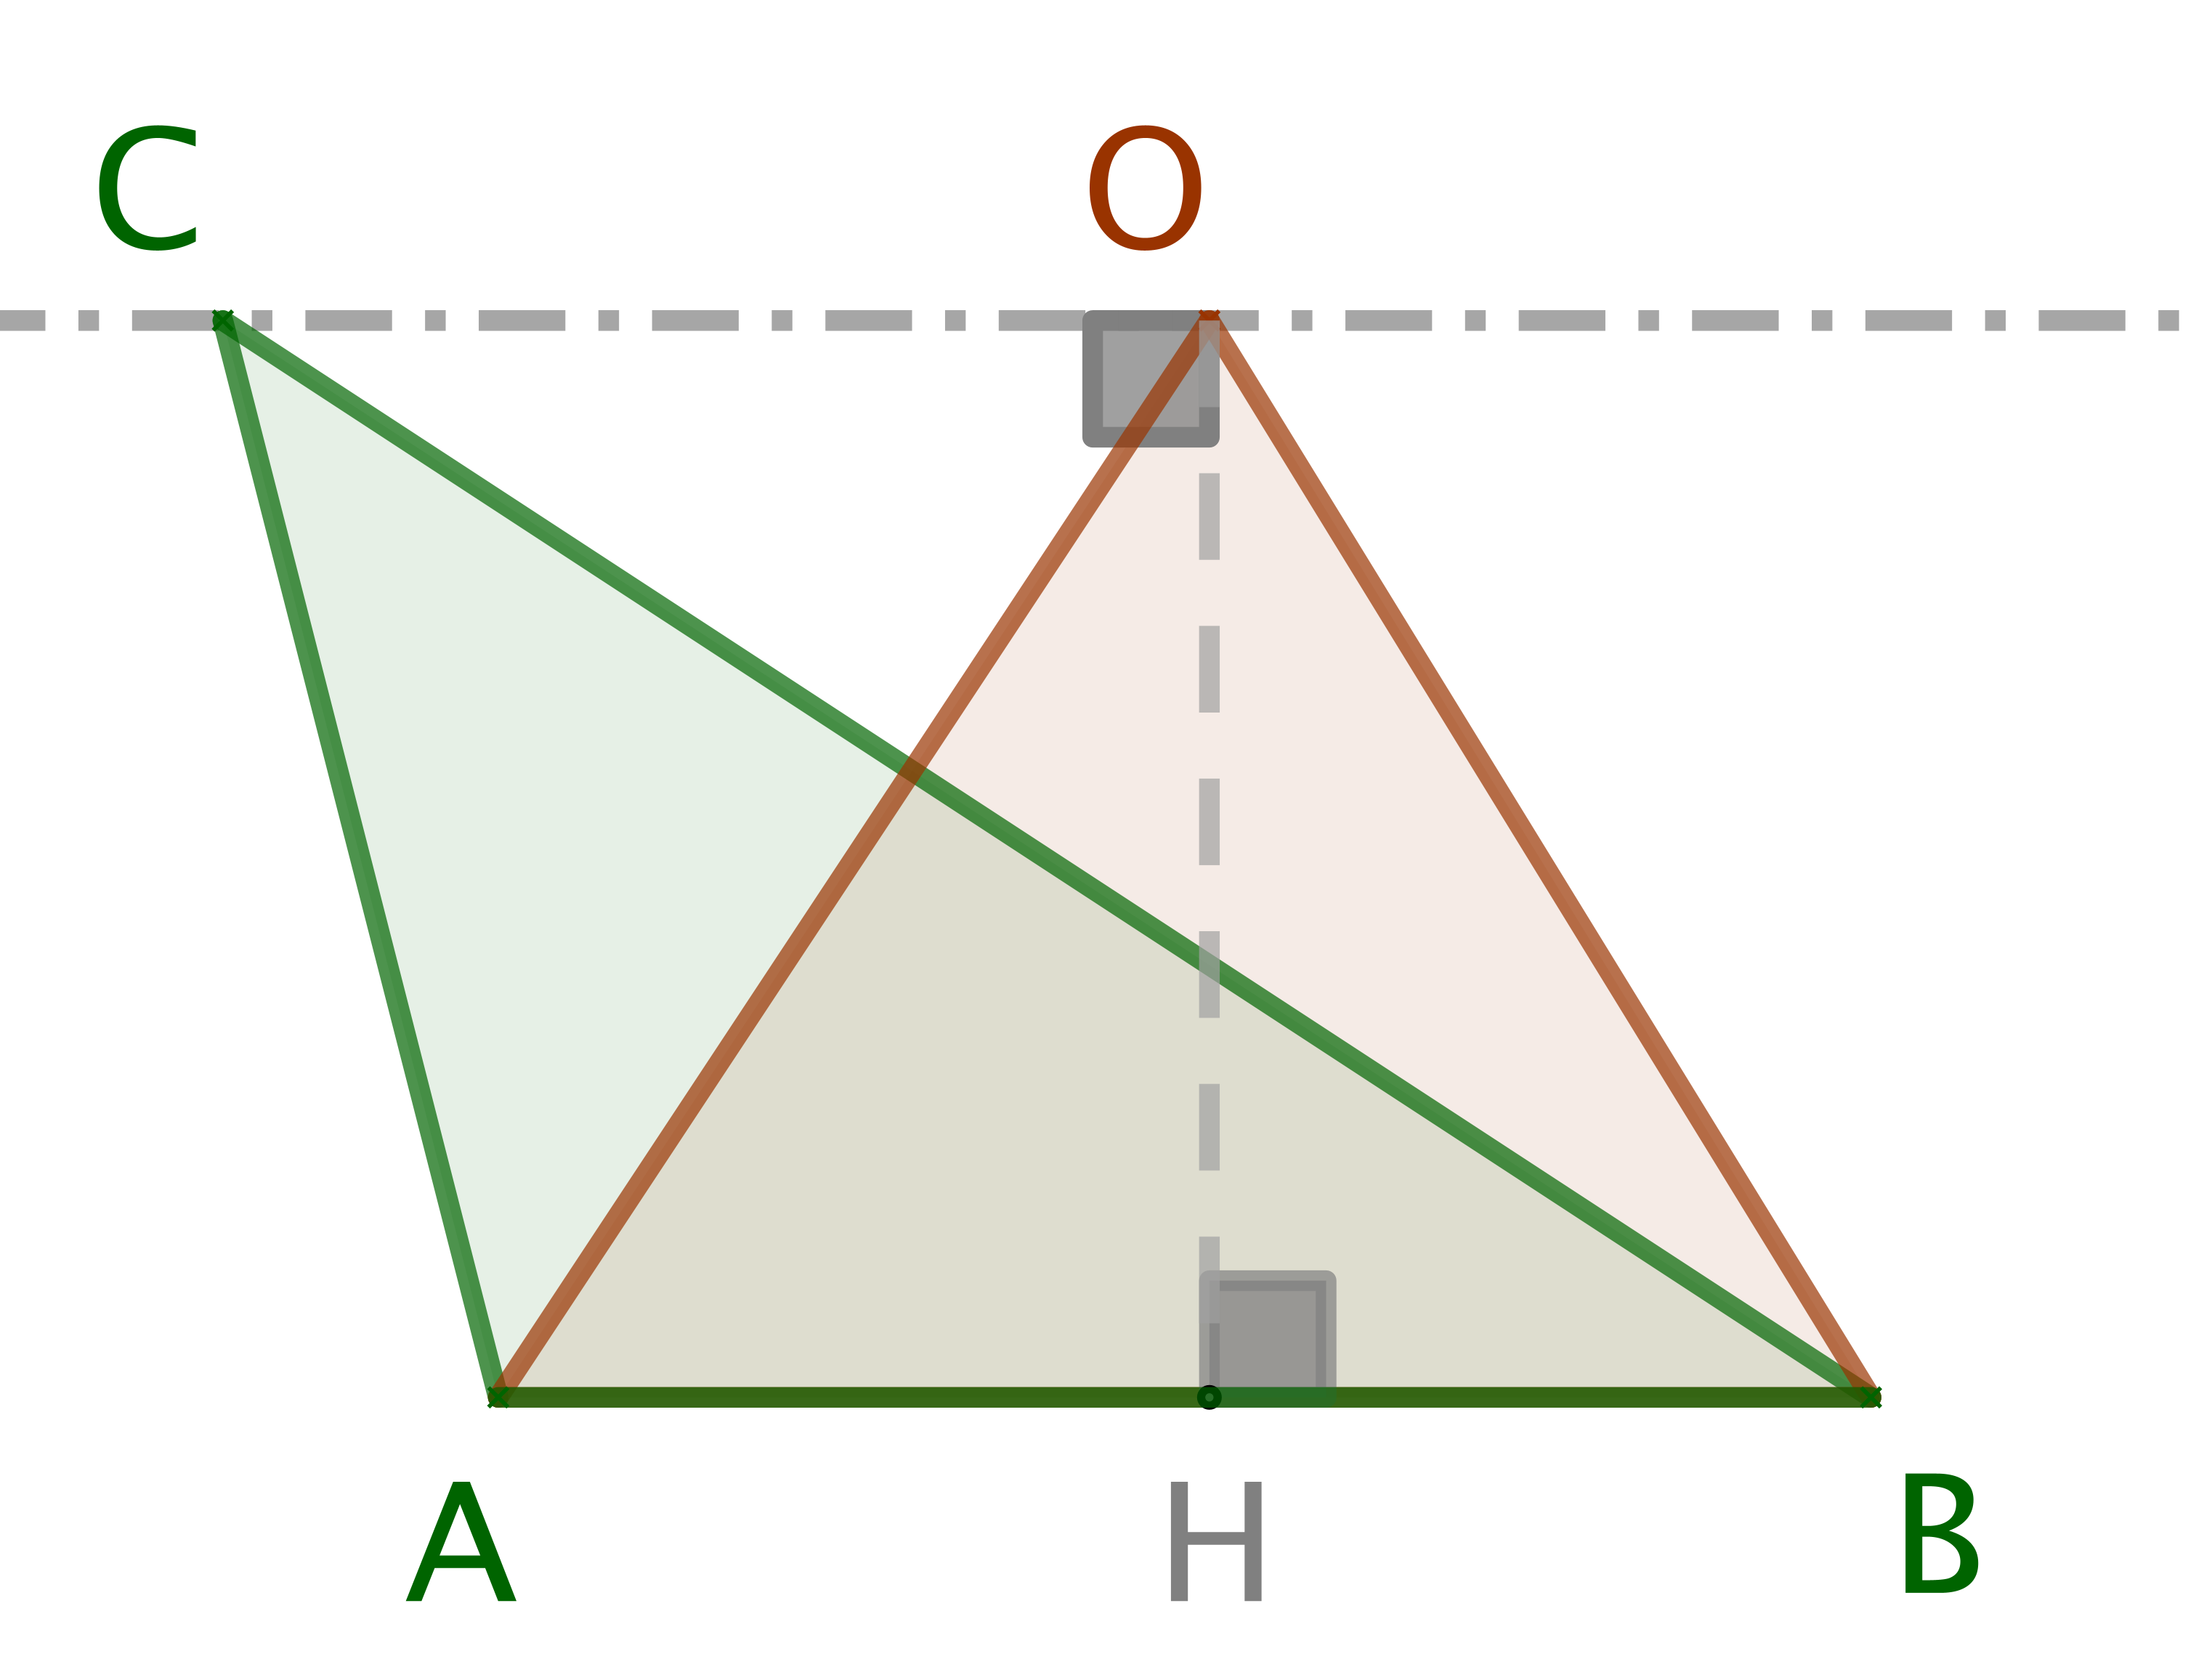
\includegraphics[scale=.4]{content/triangle-one-side-fixed/triangle.png}
	\end{center}

	
	Via une petite symétrie axiale, voir ci-dessous, il est aisé de noter que $\perim{ABC} \geq \perim{ABO}$, avec égalité uniquement si $ABC$ est isocèle en $C$. 
	
	\begin{center}
		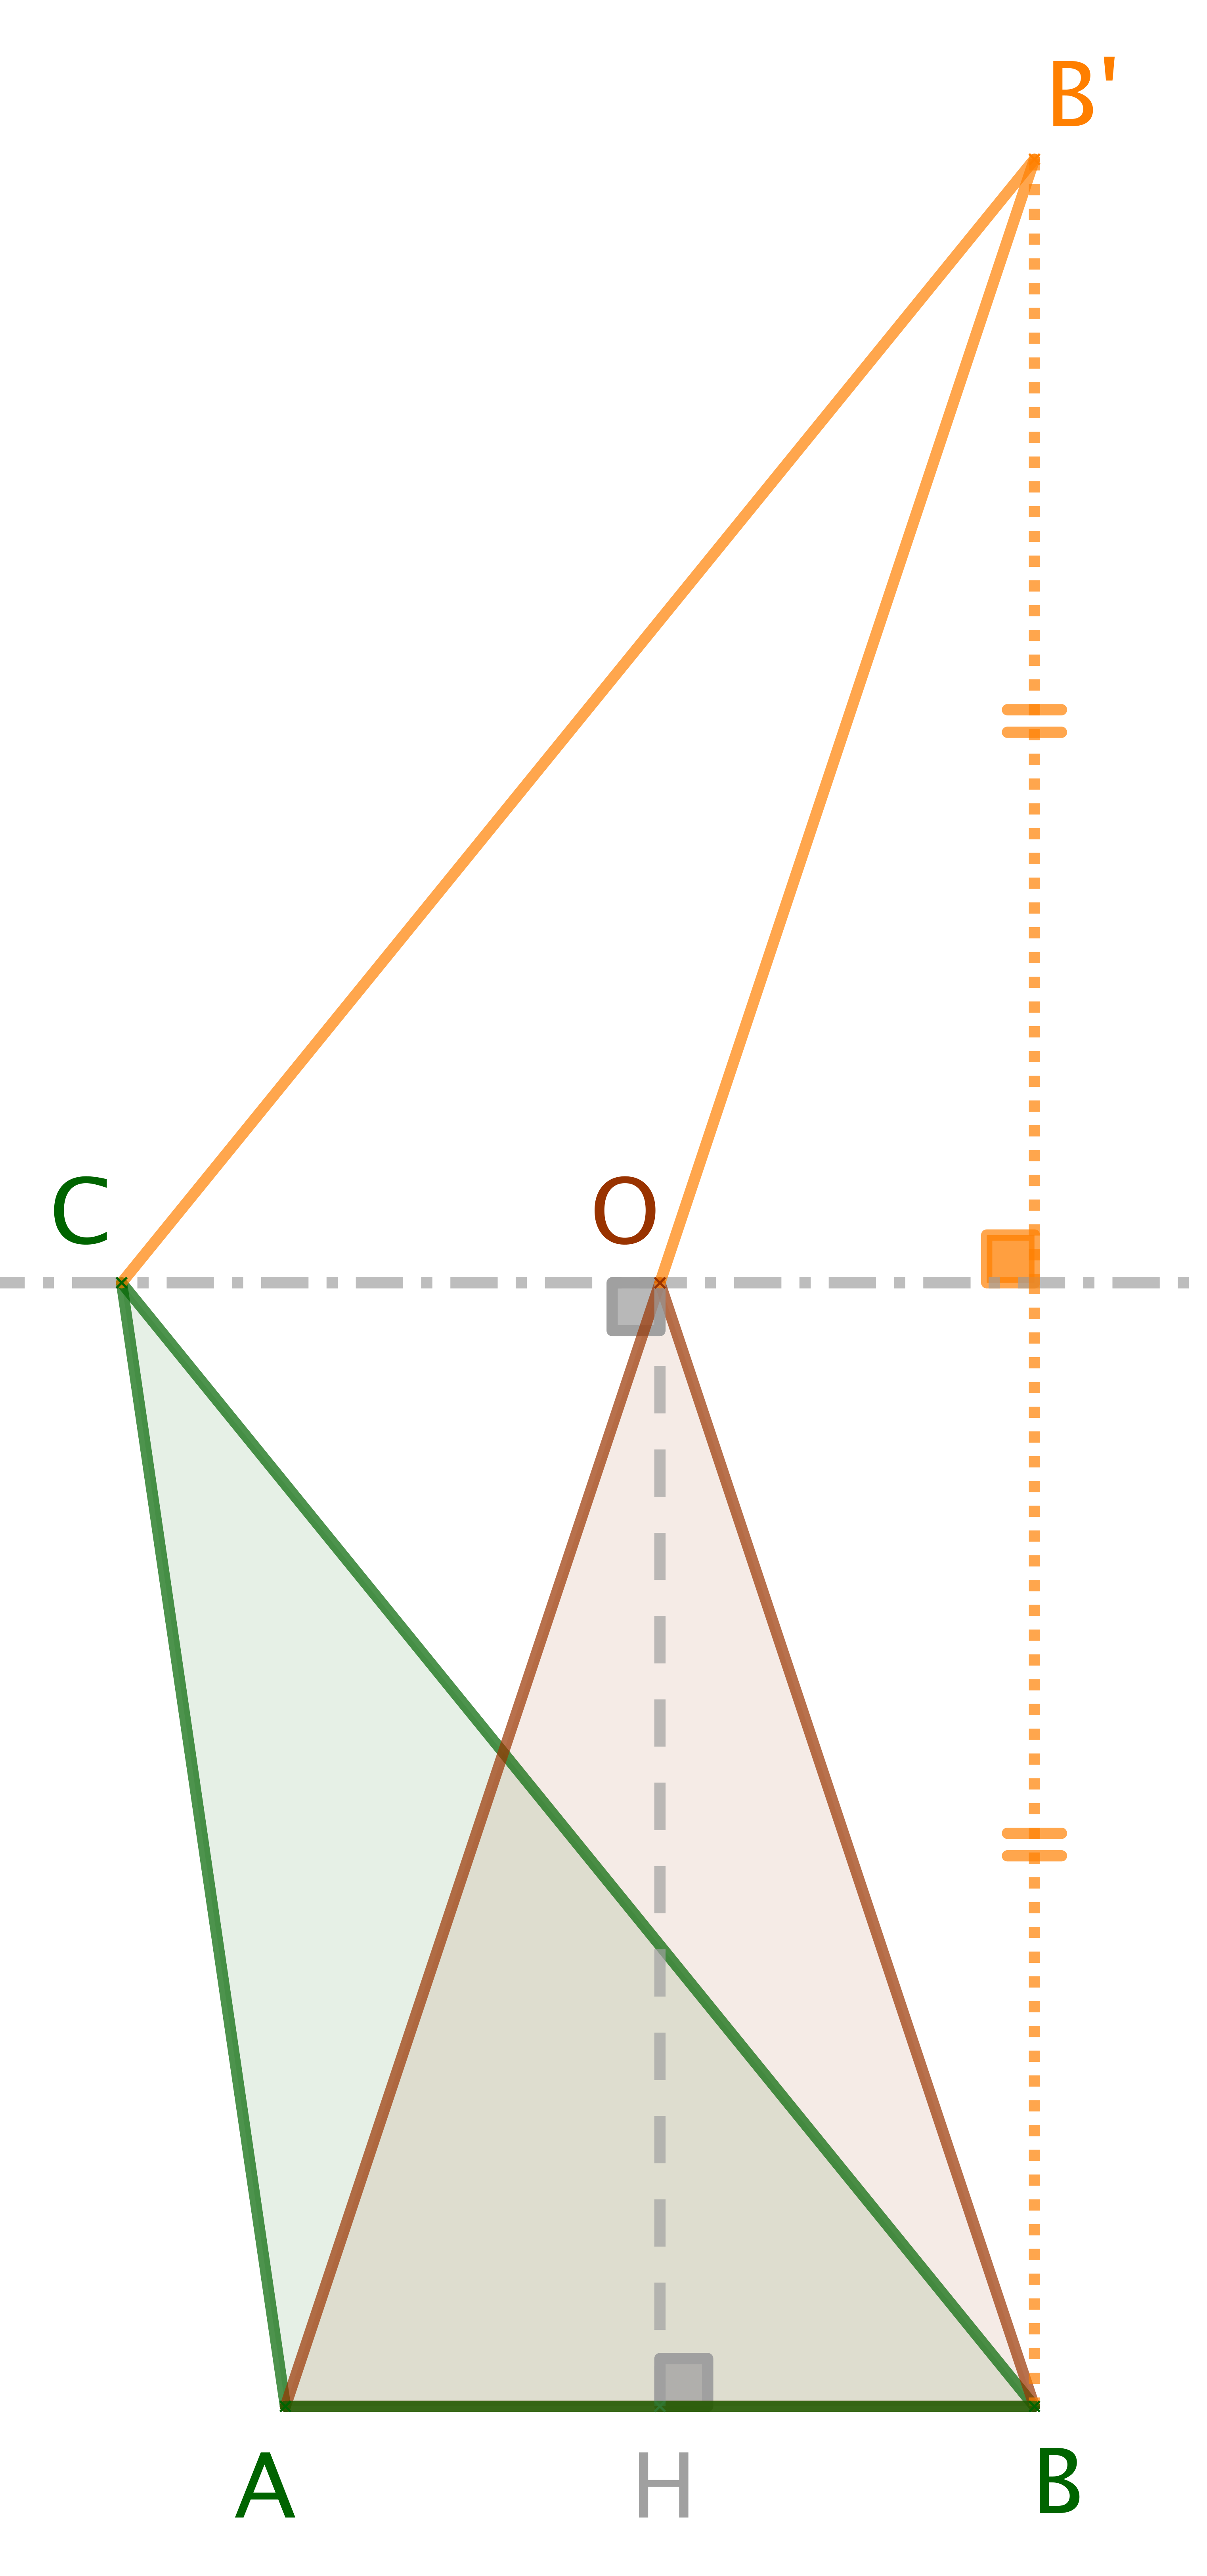
\includegraphics[scale=.4]{content/triangle-one-side-fixed/triangle-proof.png}
	\end{center}
	
	Via une dilatation \og \emph{verticale} \fg\ de rapport $r = \frac{\perim{ABC}}{\perim{ABO}} \geq 1$, on obtient finalement un triangle isocèle $ABO^{\,\prime}$ de périmètre $p$, et qui vérifie $\area{ABO^{\,\prime}} \geq \area{ABC}$, avec égalité uniquement si $ABC$ est isocèle en $C$. 
	Contrat rempli!%
	\footnote{
		La remarque \ref{constrained-extrema} explique comment employer la méthode des extrema liés. 
		Les arguments fournis à cet endroit s'adaptent facilement au cas des triangles de base fixée.
	}
\end{proof}
